\documentclass[11pt,french]{article}
\input preambule_2013

\newcounter{exoc}
\newenvironment{exoc}[1]{%
  \refstepcounter{exoc}\textbf{Exercice \theexoc} :\hfill {\footnotesize\textbf{(#1)}}\par
  \medskip}%
{\medskip}

\pagestyle{fancy}
\pieddepage{}{\thepage}{}

\setlength{\textheight}{26cm}% Hauteur de la zone de texte

\begin{document}


\begin{center}
\begin{tabularx}{\textwidth}{|>\centering m{2.5cm}|>\centering X|>{\centering\arraybackslash} m{2.5cm}|}
	\hline
		1\iere \bsc{s.t.m.g.} &  Mercredi 30 avril \np{2014} & \textbf{Bilan annuel} \\
	\hline
		\multicolumn{3}{|c|}{\bsc{Contrôle de mathématiques}} \\
	\hline
        \multicolumn{1}{|r}{\bsc{Nom}:} & \multicolumn{2}{l|}{} \\
		\multicolumn{1}{|r}{Prénom:} & \multicolumn{2}{l|}{} \\
	\hline
        \multicolumn{3}{|l|}{\bfseries Note et observations :} \\[1cm]
    \hline
\end{tabularx}\bigskip

{\itshape
La calculatrice est \textbf{autorisée}. Les feuilles de brouillon personnelles sont \textbf{interdites}.\par
Le barème est indicatif.\par
\textbf{\bsc{Attention} !! Le sujet est à rendre avec la copie.}
}
\end{center}

%-------------------------------------------------------------------------
%        EXERCICE 1
%-------------------------------------------------------------------------

\begin{exoc}{3 points - Polynésie : juin 2013}
    \textbf{Cet exercice est un \bsc{q.c.m.}}\par
    {\small\itshape
        Pour chaque question, quatre réponses sont proposées parmi lesquelles une seule est correcte.\par
        Une réponse juste apporte un point ; une réponse fausse ou l'absence de réponse n'apporte pas de point et n'en retire pas.\par
        \textbf{Consigne importante :} Pour chaque question, reporter sur la copie le numéro de la question suivi de la réponse choisie.\par
        Aucune justification n'est demandée.
    }\medskip

    \begin{enumerate}
        \item Le cours d'une matière première a augmenté de $180\%$ en un an. Il a été :
        \begin{center}
            \begin{tabularx}{\linewidth}{*{4}{>{\centering\arraybackslash}X}}
                \textbf{a.} multiplié par $0,80$ &
                \textbf{b.} multiplié par $1,80$ &
                \textbf{c.} multiplié par $2,80$ &
                \textbf{d.} multiplié par $1,18$
            \end{tabularx}
        \end{center}

        \item Quel est le taux d'évolution réciproque de $+25\%$ ?
        \begin{center}
            \begin{tabularx}{0.9\linewidth}{*{4}{>{\centering\arraybackslash}X}}
                \textbf{a.} $-20\%$ &
                \textbf{b.} $-25\%$ &
                \textbf{c.} $-75\%$ &
                \textbf{d.} $+80\%$
            \end{tabularx}
        \end{center}

        \item Le prix d'un bien d'équipement augmente de $5\%$ la première année puis diminue de $2\%$ la seconde année.\par
        Le taux d'évolution sur les deux années est, à $0,01\%$ près :
        \begin{center}
            \begin{tabularx}{0.9\linewidth}{*{4}{>{\centering\arraybackslash}X}}
                \textbf{a.} $+1,50\%$ &
                \textbf{b.} $+3,49\%$ &
                \textbf{c.} $+1,44\%$ &
                \textbf{d.} $+2,90\%$
            \end{tabularx}
        \end{center}
    \end{enumerate}
\end{exoc}
\[*\]

%-------------------------------------------------------------------------
%        EXERCICE 2
%-------------------------------------------------------------------------

\begin{exoc}{6 points - Nouvelle-Calédonie : mars 2014}
    Une émission de télé-réalité est diffusée une fois par semaine. On désire, dans cet exercice, étudier les audiences de cette émission sur un groupe de $\np{1000}$ adolescents. La première semaine, $400$ adolescents de ce groupe ont regardé l'émission.\par\smallskip
    On note $u_n$ le nombre d'adolescents du groupe ayant regardé l'émission la $n$-ième semaine. \par Ainsi, le premier terme est $u_1$.

    \begin{enumerate}
        \item En utilisant l'énoncé, donner la valeur de $u_1$.
    \end{enumerate}

    On estime que les audiences augmentent chaque semaine de $5\%$.

    \begin{enumerate}[resume]
        \item Calculer la valeur de $u_2$ puis de $u_3$.
        \item Donner l'expression de $u_{n+1}$ en fonction de $u_n$.
        \item Quelle est la nature de la suite $(u_n)$ ? Justifier.
        \item Exprimer $u_n$ en fonction de $n$.
        \item La finale de cette émission se déroule la douzième semaine.\par
        À l'aide de la calculatrice, donner le nombre d'adolescents ayant regardé la finale. Arrondir le résultat à l'unité.
    \end{enumerate}
\end{exoc}
\[*\]\clearpage

%-------------------------------------------------------------------------
%        EXERCICE 3
%-------------------------------------------------------------------------

\begin{exoc}{7 points - Métropole : juin 2013}\label{benefice}
Un artisan fabrique des meubles qu'il vend au prix de $150$ euros l'unité. Chaque semaine, il en produit maximum $16$. On suppose que l'artisan vend tous les meubles qu'il fabrique.\par
Le coût de fabrication de $x$ meubles, charges de l'entreprise incluses, exprimé en euros, est noté $C(x)$. La fonction $C$ est définie sur l'intervalle $\intervalleff{1}{16}$.\medskip

%----------------------------------------------------------------------------
\textbf{Partie} \rond{A}\quad Lectures graphiques\medskip
%-----------------------------------------------------------------------------

Dans le graphique donné en annexe page \pageref{Annexe}, on a représenté la fonction de coût $C$ et la fonction recette $R$ respectivement par les courbes $\calig C$ et $\calig R$.\par
Répondre aux questions suivantes par des phrases complètes en utilisant le graphique.\par
\textit{On laissera apparents les traits nécessaires à cette lecture graphique.}

\begin{enumerate}
    \item Quel est le coût de fabrication de $6$ meubles, exprimé en euros ?\par Quel est le coût de fabrication de $13$ meubles, exprimé en euros ?
    \item Est-il rentable pour l'artisan de fabriquer et vendre $13$ meubles ? Justifier la réponse.
    \item Pour un coût de fabrication de $900$ euros, combien l'artisan fabrique-t-il de meubles ?
    \item Déterminer les nombres de meubles qui doivent être fabriqués pour que l'entreprise soit bénéficiaire.
\end{enumerate}\medskip

%----------------------------------------------------------------------------
\textbf{Partie} \rond{B}\quad \'Etude du bénéfice\medskip
%----------------------------------------------------------------------------

Le bénéfice est donné par $B(x)$ où $B$ est la fonction définie sur l'intervalle $\intervalleff{1}{16}$ par :\[B(x) = -10x^2 + 140x - 180.\]

\begin{enumerate}
    \item Donner le tableau de variations de $B$ sur $\R$.
    \item Pour combien de meubles fabriqués et vendus le bénéfice est-il maximal ? Justifier à l'aide d'un calcul.
    \item Calculer alors ce bénéfice maximum.
    \item Déterminer les solutions de l'équation $B(x) = 0$. Arrondir les solutions au dixième près.
\end{enumerate}

\end{exoc}\[*\]

%-------------------------------------------------------------------------
%        EXERCICE 4
%-------------------------------------------------------------------------

\begin{exoc}{4 points - Antilles-Guyane : septembre 2013}\label{proba}
    Une boîte de biscuits contient $80$ biscuits d’aspect identique.\par
    On sait que, dans cette boîte :
        \begin{itemize}[label=\textbullet\quad]
            \item $40$ biscuits sont à la vanille, $24$ biscuits sont à l’orange et les biscuits restants sont à la noix de coco ;
            \item $60\%$ des biscuits à la vanille contiennent des pépites de chocolat ;
            \item $25\%$ des biscuits à l’orange contiennent des pépites de chocolat ;
            \item Aucun biscuit à la noix de coco ne contient de pépites de chocolat.
        \end{itemize}
    La boite étant pleine, on choisit au hasard un biscuit dans la boîte. On admet que chaque biscuit a la même probabilité d’être choisi.\par\smallskip
    On définit les évènements suivants :\par
    $V$ : << le biscuit choisi est un biscuit à la vanille >> ;\par
    $O$ : << le biscuit choisi est un biscuit à l’orange >> ;\par
    $N$ : << le biscuit choisi est un biscuit à la noix de coco >> ;\par
    $C$ : << le biscuit choisi contient des pépites de chocolat >>.\par\smallskip
    Pour tout évènement $A$, on note $\overline A$ l’évènement contraire de $A$ et $p(A)$ la probabilité que l’évènement $A$ soit réalisé.\par
    Dans les questions suivantes, les probabilités seront données \textbf{sous forme décimale}.\medskip

    \begin{enumerate}
        \item Justifier que la probabilité que l’on choisisse un biscuit à la noix de coco est égale à $0,2$.
        \item Compléter l’arbre pondéré représentant la situation donné en annexe page \pageref{Annexe}.
        \item Définir par une phrase l’évènement $V \cap C$ et calculer sa probabilité.
        \item Montrer que : $p(C)= 0,375$.
    \end{enumerate}
\end{exoc}


\clearpage

\begin{center}\label{Annexe}
    \Large\bfseries
    Annexe
\end{center}

\begin{center}
\textbf{Exercice \ref{benefice}}\medskip

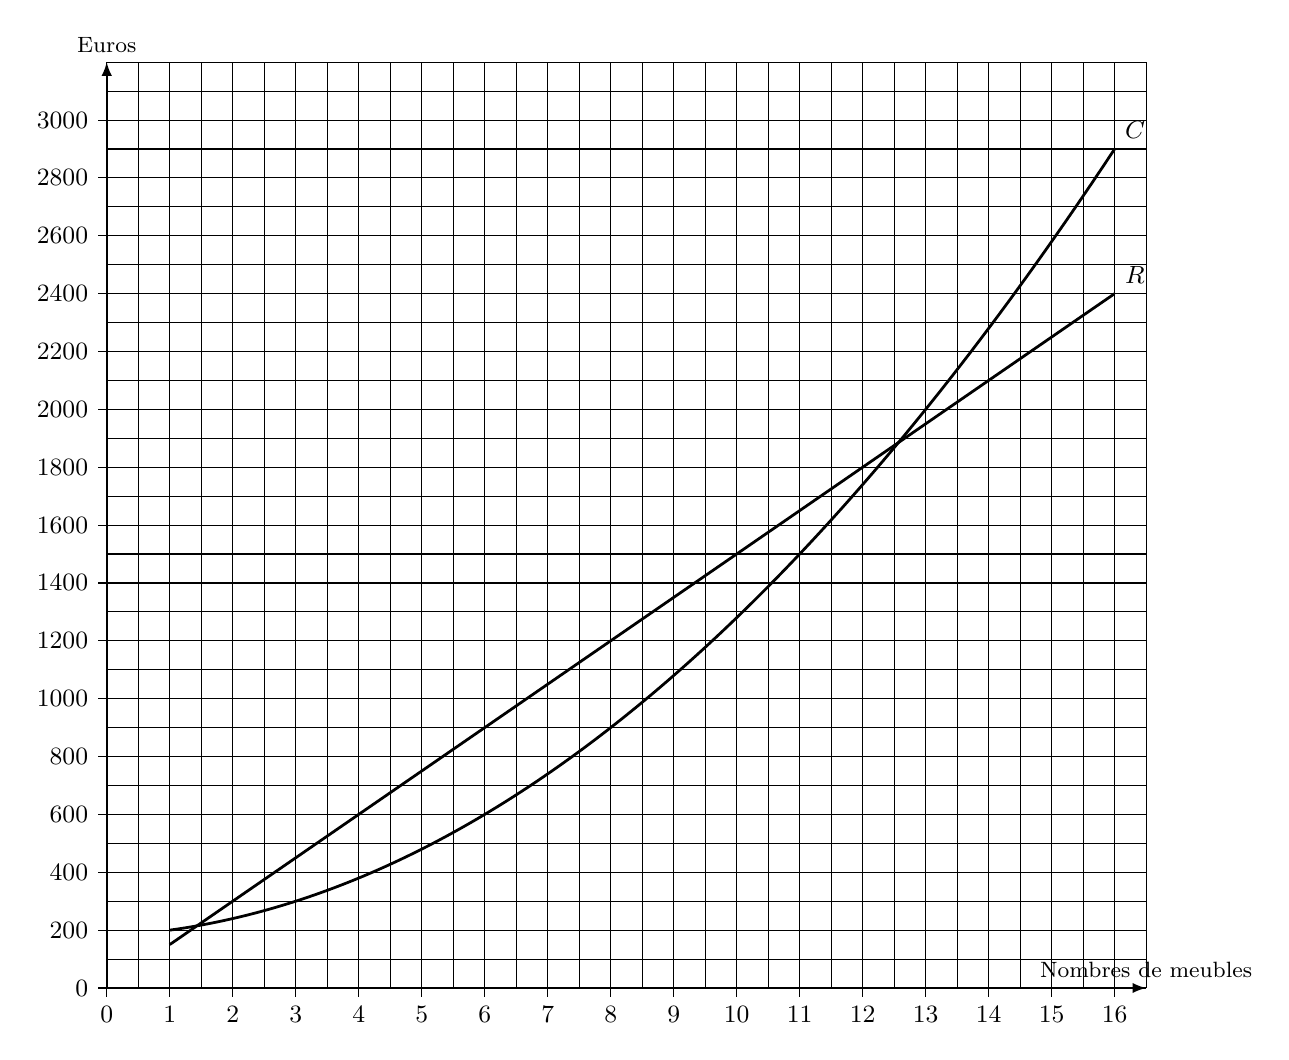
\begin{tikzpicture}[>=latex,x=1cm,y=0.0046cm,scale=0.8]
    \draw[line width = 0.4pt] (0,0) grid[xstep=0.5,ystep=100] (16.5,3200);
    \draw[->,line width=0.7pt] (0,0) -- (16.5,0) node[above] {\footnotesize Nombres de meubles};
    \draw[->,line width = 0.7pt] (0,0) -- (0,3200) node[above] {\footnotesize Euros};
    \draw[line width=1pt] plot[domain=1:16,samples=200] (\x,{150*(\x)}) node[above right]{\small $\calig R$};
    \draw[line width=1pt] plot[domain=1:16,samples=200] (\x,{10*(\x)^2+10*\x+180}) node[above right]{\small $\calig C$};
    \foreach \x in {0,...,16} \draw (\x,0)--(\x,-4pt) node[below] {\small $\x$};
    \foreach \x in {0,200,...,3000} \draw (0,\x)--(-4pt,\x) node[left] {\small $\x$};
\end{tikzpicture}
\end{center}\medskip

%---- On définit ci-dessous les différents styles en fonction du niveau dans l'arbre de proba :
\tikzstyle{level 1}=[level distance=2cm,sibling distance=-3cm]
\tikzstyle{level 2}=[level distance=2.5cm,sibling distance=-1.5cm]

%---- sibling distance négative => les noeuds sont compilés de haut en bas

\begin{center}
\textbf{Exercice \ref{proba}}\vspace{1cm}

    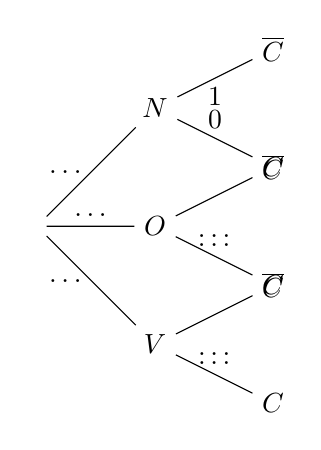
\begin{tikzpicture}
    [grow=right] % dessine l'arbre de gauche à droite. Les options left, up et down sont également disponibles.
        \node{}
    %----------------------------------------------------------------------------------------------------------------------
    %----------------------------------------------------------------------------------------------------------------------
            child {node {$V$}
    %----------------------------------------------------------------------------------------------------------------------
                    child {node {$C$}
                             edge from parent node[above] {$\ldots$}
                            }
    %----------------------------------------------------------------------------------------------------------------------
                    child {node {$\overline C$}
                             edge from parent node[below=10pt] {$\ldots$}
                            }
    %----------------------------------------------------------------------------------------------------------------------
               edge from parent node[left] {$\ldots$}
            }
    %----------------------------------------------------------------------------------------------------------------------
    %----------------------------------------------------------------------------------------------------------------------
            child {node {$O$}
    %----------------------------------------------------------------------------------------------------------------------
                    child {node {$C$}
                             edge from parent node[above] {$\ldots$}
                            }
    %----------------------------------------------------------------------------------------------------------------------
                    child {node {$\overline C$}
                             edge from parent node[below=10pt] {$\ldots$}
                            }
    %----------------------------------------------------------------------------------------------------------------------
                edge from parent node[above] {$\ldots$}
            }
    %----------------------------------------------------------------------------------------------------------------------
    %----------------------------------------------------------------------------------------------------------------------
            child {node {$N$}
    %----------------------------------------------------------------------------------------------------------------------
                    child {node {$C$}
                             edge from parent node[above] {$0$}
                            }
    %----------------------------------------------------------------------------------------------------------------------
                    child {node {$\overline C$}
                             edge from parent node[below] {$1$}
                            }
    %----------------------------------------------------------------------------------------------------------------------
                edge from parent node[left] {$\ldots$}
            }
    ;
    \end{tikzpicture}
\end{center}

\end{document} 